% !tex root = ../Thesis.tex

This chapter describes the design, module implemetation and final implemetations
of the pitch correction system. The implementation code was written in Octave, a
free and open source alternative to Matlab. Some important, short code-snips are
shown and explaind to give deeper insight into the details of the implementation.

Since one of the goals of this report is to compare the performance of the pitch
corrector when using different modules, the evaluation metrics used are described
first. Theses metrics are described first to reflect the fact that the metrics
were designed before the structure and submodules were implemented in an effort to
minimise biased results. Once these metrics are well understood, the desing and
implementation of the pitch corrector and its submodules are described.

\section{Evaluation Metrics Design}

The goal of using metrics is to give a meaningful quantitative way of measuring
the success of the pitch corrector. It provides way to compare the performance of
different sub modules and choose the configuration that produces the best result.
Since the ultimate goal of an audio pitch corrector is to produce better sounding
music, the most rigorous way to judge the effectiveness of the pitch corrector
would be to run a psychological survey on which combination of sub modules sound
best. This is beyond the scope of this project. Instead, some simplifications are
made and metrics are designed based on the research done on music theory. These
metrics act as a proxy for the results given by a physiological survey and are
much easier and cheaper to run. Two aspects of the pitch corrector are chosen to
be assessed. The effectiveness of it and the noise or distortion of the audio
signal introduced by the pitch corrector.

\subsection{Pitch Corrector Metrics}

The effectiveness metric is a way of measuring how much the pitch corrector
corrects the pitch. This metric will answer the question of how in tune the audio
is before and after the correction is applied and produce a number indicating the
improvement. The algorithm to achieve this will make use of the frequency contour
function. This is a function of the fundamental frequency of a signal over time.
Exactly how the frequency contour is extracted from the signal will be discussed
in the ``Pitch Correction Design'' section. From this frequency contour function,
it is possible to find the closest correct frequency to this function as shown in
listing \ref{lst:getClosestFreqContour}.\octavelisting{getClosestFreqContour} The
exact details of how the correct frequencies are calculated will be explained in
the ``Target Frequency Contour'' section. Listing \ref{lst:getClosestFreqContour}
shows how the closest frequency contour is calculated.

Once the closest frequency contour is found, both are converted into a pitch
contour by taking the $log_2$ of the functions. This is done because using
frequency contours would eventually weigh the importance of the higher frequencies
more than the lower frequencies. A plot of these two contours would allow one to
see the intonation error as shown in figure \ref{fig:ErrorFunction}.

\begin{figure}[h]
	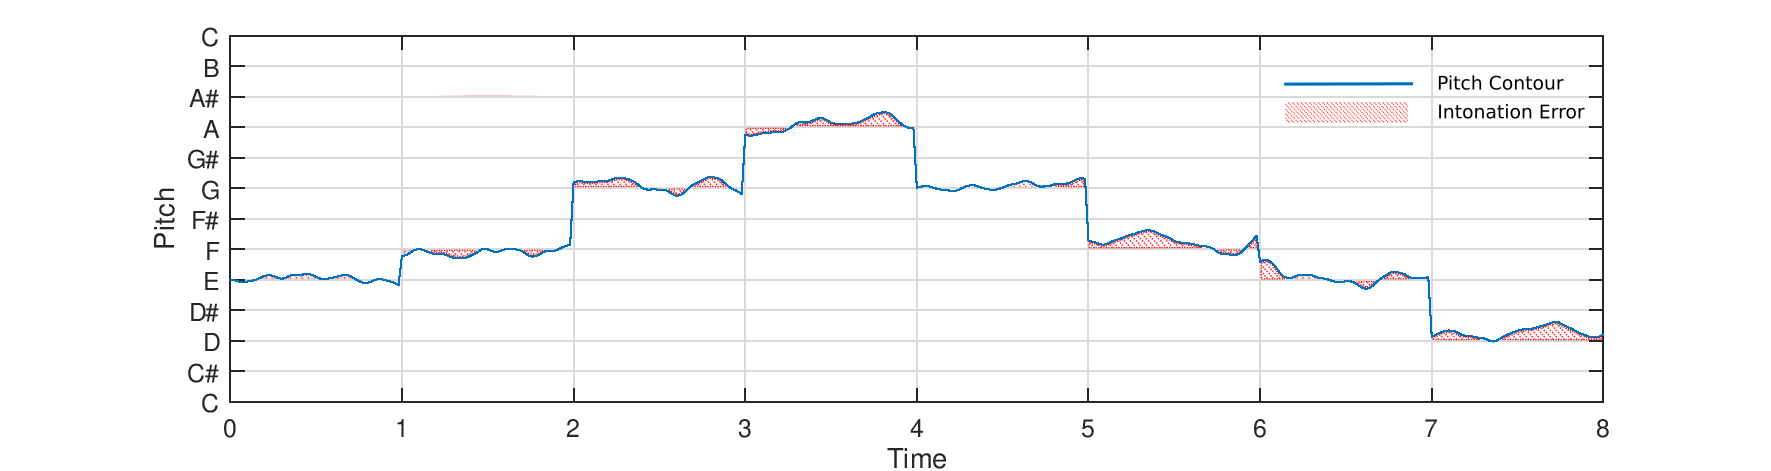
\includegraphics[width=\textwidth,trim={3.5cm 0cm 2.8cm 0cm}]
	{IntonationError}
	\caption{Illustration of Intonation Errors in a Pitch Contour Diagram}
	\label{fig:ErrorFunction}
\end{figure}

The red regions in figure \ref{fig:ErrorFunction} are intonation errors. To be
perfectly in tune would be saying there are no red regions, or equivalently, the
error function is zero everywhere. Therefore the smaller the red regions are the
better the pitch corrector. A common metric to measure this is the mean square
error metric and even has a built-in function in Octave. Therefore the mean square
error would indicate how in tune the audio recording is, weighing larger
intonation errors greater than small intonation errors. This metric is referred to
as the mean squared pitch error and can fundamentally not be greater than
$1.736\times10^{-3}$ in the equal tempered tuning system. How this number is
calculated is shown in equation \ref{eq:MaxIntonationError} and is essentially
half the distance between two notes in the logarithmic pitch scale.

\begin{equation}\label{eq:MaxIntonationError}
	\bigg(\frac{1}{2}log_2(\sqrt[12]{2}) - log_2(1)\bigg)^2 \approx
	1.736\times10^{-3}
\end{equation}

To formalise this metric algorithm, a standard recording needs to be chosen to
test with. An exponential chirp signal is chosen, starting at 110Hz, ending at
440Hz and lasting 5 seconds. Figure \ref{fig:ChirpContour} shows the pitch contour
of the signal with the closest correct pitch contour. This signal has a mean
squared pitch error of $0.59 \times 10^{-3}$. The algorithm will measure the
mean squared pitch error after the pitch correction is applied and return a ratio
of the original and corrected mean squared pitch error. The idea being that the
metric essentially says the pitch correction effect causes the recording to be X
times more in tune. The goal of the pitch corrector is to maximise this metric.

\begin{figure}[h]
	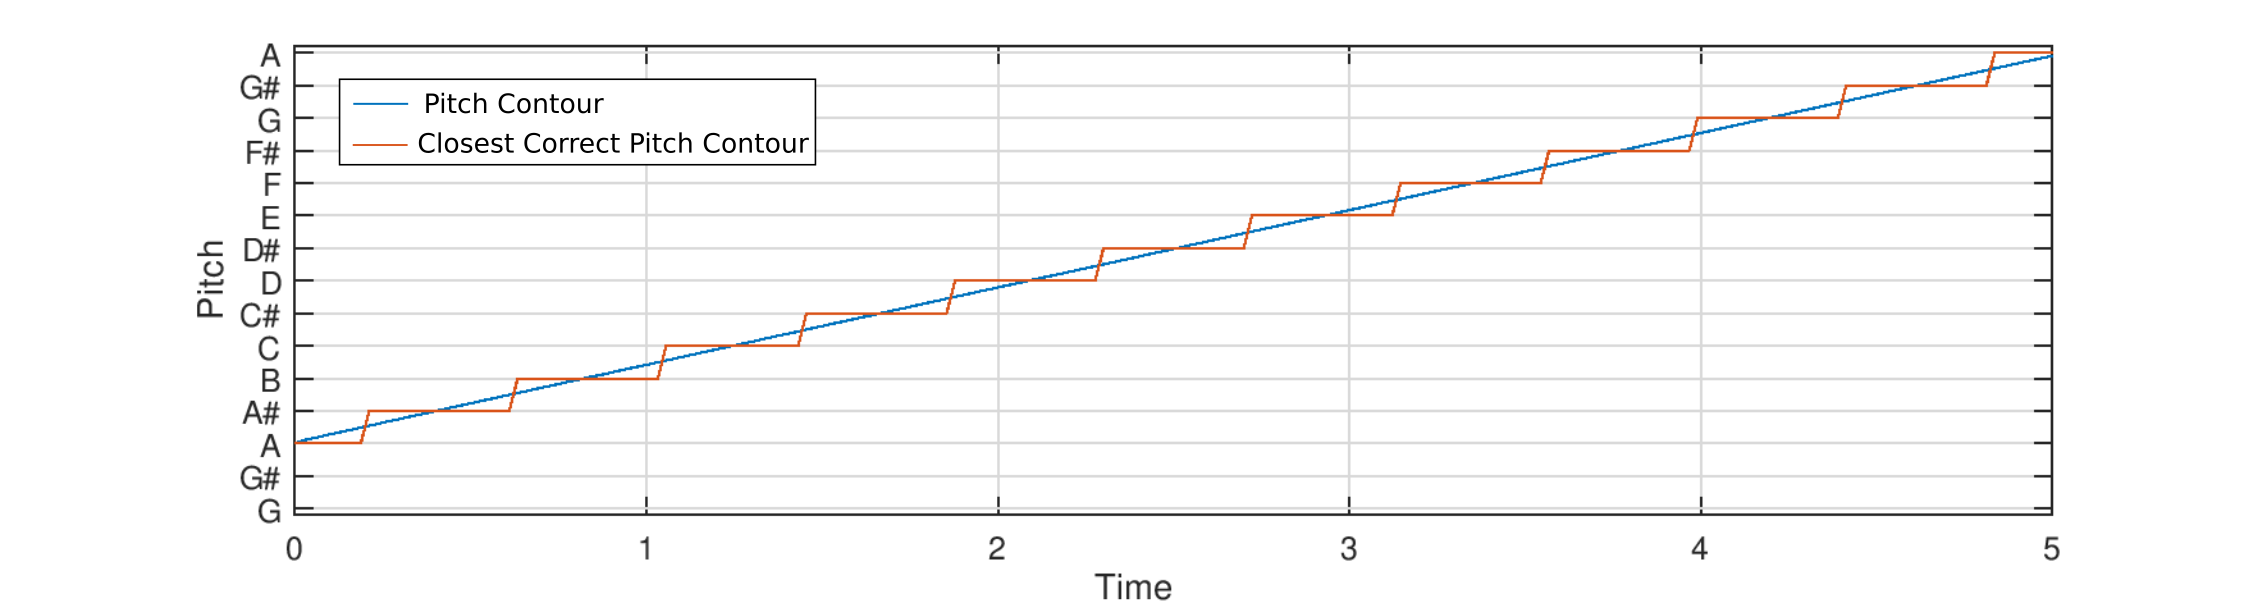
\includegraphics[width=\textwidth,trim={3.5cm 0cm 2.8cm 0cm}]
	{ChirpContour}
	\caption{Exponential Chirp Contour with Closest Frequency Contour}
	\label{fig:ChirpContour}
\end{figure}

The effectiveness metric unfortunately relies on the frequency detector to be
absolutely correct. This is because it depends on the results of the frequency
contour before and after the correction was made. The choice to use a clean chirp
signal for this metric was made to minimise dependence on the frequency detector.

Now that the effectiveness of the pitch corrector can be measured, a distortion
metric needs to be designed to measure how much the pitch corrector distorts the
signal unnecessarily. The idea is to have a signal in a state that it shouldn't
require a correction anymore, i.e. Already pitch corrected, and then apply the
pitch correction effect and see how much the signal change. The idea is to measure
the peak of the autocorrelation of a signal after applying the pitch correction
effect. This is the baseline value. Then apply the pitch correction effect again
and calculate the maximum value of the cross-correlation between the signal before
and after the second pitch correction effect has been applied. The ratio between
the maximum cross-correlation value and the baseline value gives in indication to
how much the pitch corrector distorts the signal unnecessarily. This ratio is
called the distortion metric, measured as a percentage. A pitch correction
algorithm will attempt to produce the highest similarity ratio, 100\% being a
perfect score. Listing \ref{lst:distortionMetric} shows the distortion metric
algorithm implemented in Octave.

\octavelisting{distortionMetric}

The testing recording for the distortion metric is chosen to be the same as the
one for the effectiveness metric except for one thing. The distortion signal needs
some added white noise to have the distortion in the whole frequency range
accounted for. To avoid the white noise from interfering with the frequency
detector, the level is set to \color{red}XX\color{black}db since both the
detectors are shown to be robust enough to that level of noise in the next
section.

\subsection{Noise Robustness Metric}

As has already been mentioned, the effectiveness metric relies on the fact that
the frequency detector is absolutely correct. To give some sense that the
frequency detector is capable of producing valid results, a metric is designed to
measure how much noise the frequency detector can deal with before producing
unacceptable results. Unacceptable results are seen as a mean square error of more
than $0.59 \times 10^{-6}$, i.e. three orders of magnitude greater than the mean
squared error of the testing signal in figure \ref{fig:ChirpContour}. The testing
signal will be the  same as the one in figure 3.2 since the exact pitch contour of
the signal is known. The metric will produce a db level of noise that can be added
before the unacceptable mean squared error value has been reached. The goal of the
pitch detector would be to maximise this db level of noise added.

\section{Pitch Corrector Design}

The design of the pitch corrector is guided by what was found in the literature
review. Specifically the ``General Pitch Correction Structure'' section was found
useful. All the pitch correctors investigated had a modular design that included a
frequency detector and a frequency scaler. Some extra modules, unique to a
specific pitch corrector, were mostly ignored in the pursuit of simplicity. The
``pitch manipulation'' and ``target pitch'' modules represents essentially the
same function and was named the ``Target Frequency Contour'' module.

This chapter describes the general structure of the pitch corrector first,
explaining how the data flows through the pitch corrector. Thereafter the concept
of segmentation is explained and the exact details of how the pitch contour is
calculated is laid out.

\subsection{Structure}

The overall structure of the pitch corrector can be represented in a flow diagram.
This structure is shown in figure \ref{fig:PitchCorrectorFlowDiagram}. The blocks
represent modules that receives inputs and produces outputs. The arrows represents
the data and is labeled according to what kind of data it is, pointing in the
direction the data flows. The overall structure receives untuned audio and
produces tuned audio.

\begin{figure}[h!]
\centering
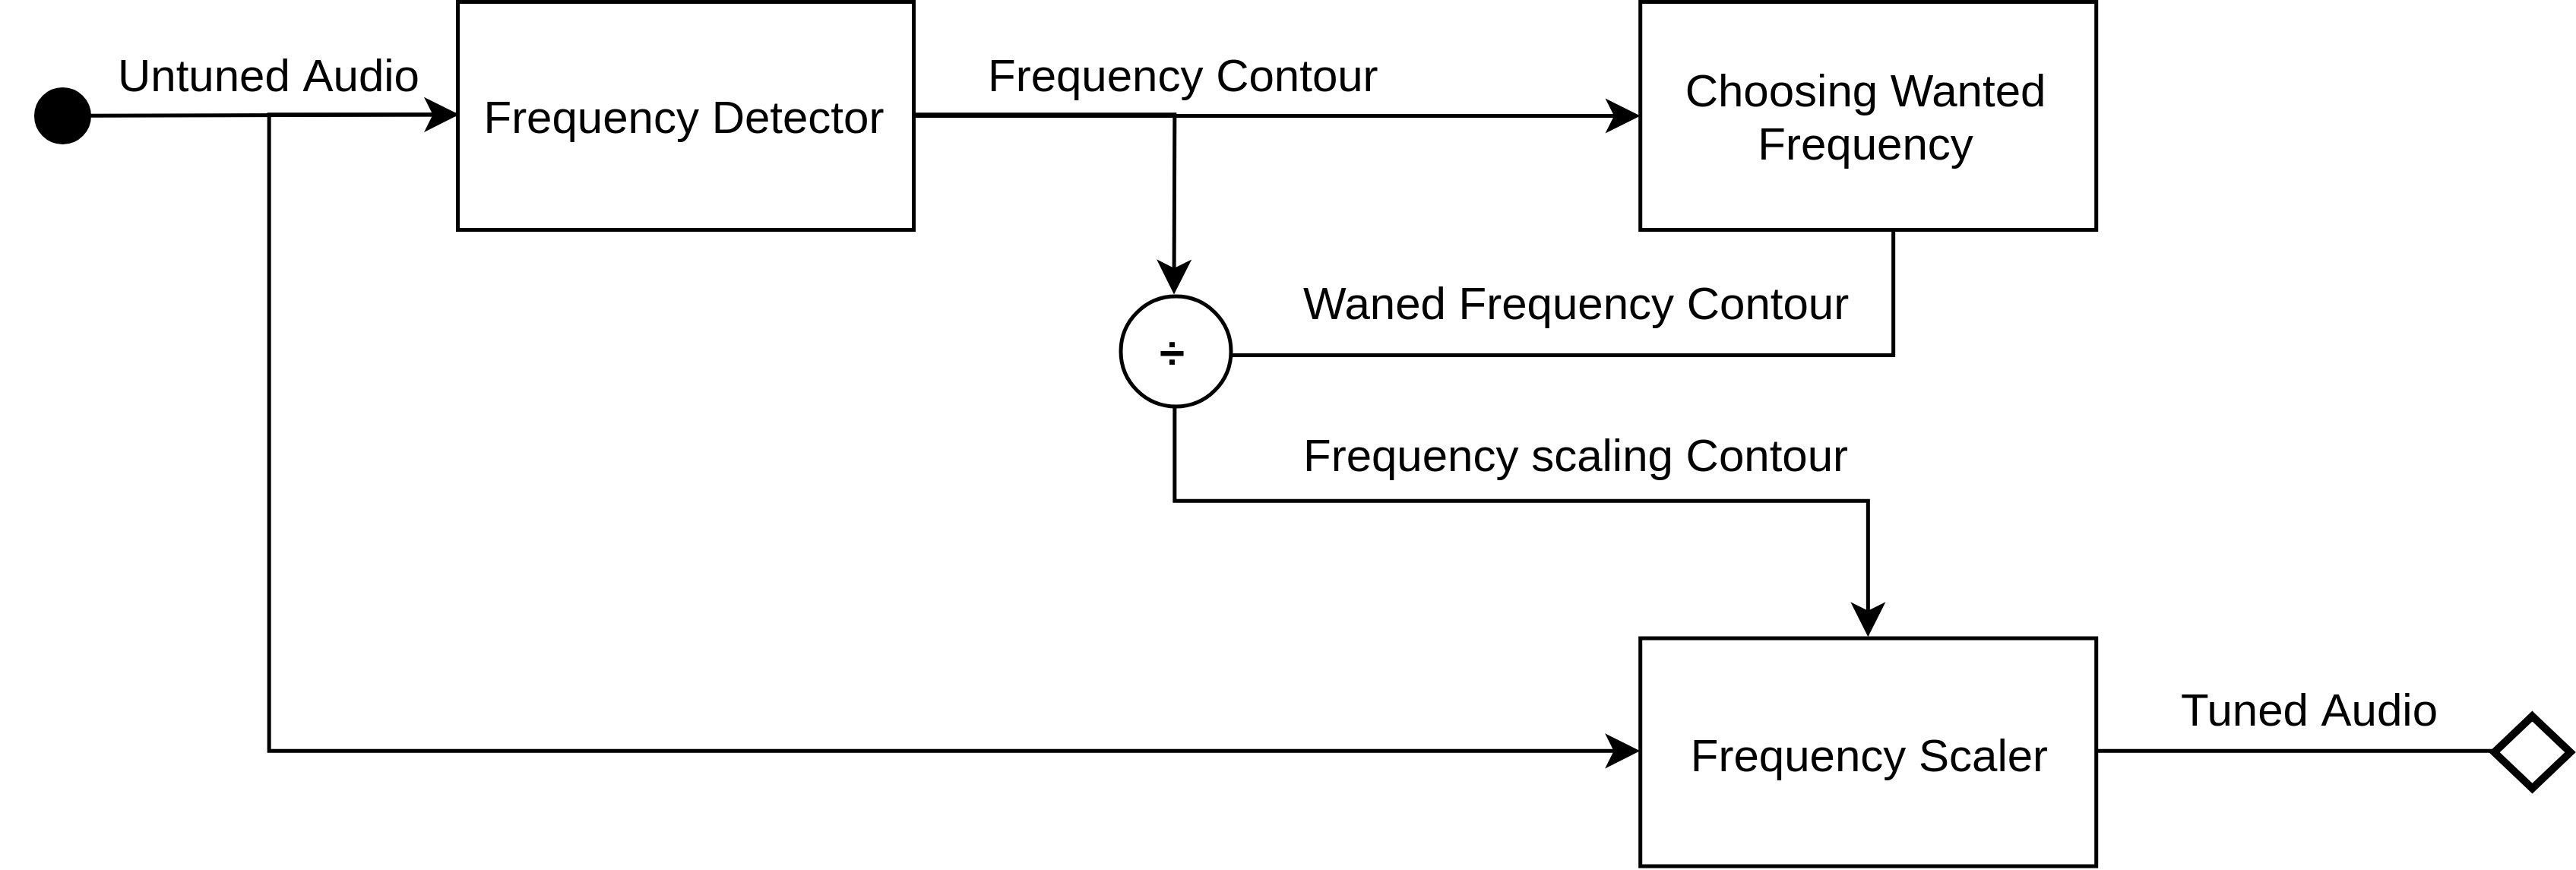
\includegraphics[width=\textwidth]{PitchCorrectorFlowDiagram}
\caption{Flow Diagram of Pitch Corrector}
\label{fig:PitchCorrectorFlowDiagram}
\end{figure}

\lstset{language=Octave}

The Octave code of the structure seen in figure
\ref{fig:PitchCorrectorFlowDiagram} can be seen in listing
\ref{lst:getCorrectedPitch}. From this code, it can be seen that some extra
information, other than that provided by the arrows, are needed. This information
includes the sampling frequency, the segment size and the hop size and is needed
by each module to function correctly. The sampling frequency is self explanatory
but segment size and hop size relates to the concept of segmentation, not yet
explained. This extends naturally to the idea of a frequency contour and is why
the wrapper function \colorbox{backcolour}{\lstinline{getFrequencyContour}}
exists, providing an intermediate step to the frequency detection module.

\octavelisting{getCorrectedPitch}

\subsection{Segmentation}

Segmentation is a concept required by the structure of the pitch corrector. It
essentially involves breaking up the input signal into segments, and doing
computations on these individual segments. The frequency detector and frequency
scaler performs it's operation in the context of a single segment. The idea of
segmentation can be seen in figure \ref{fig:Segmentation}. The figure shows a
signal being segmented into chunks of 2 048 samples and a 50\% overlap. This
corresponds to a segment duration of around 46ms, assuming a sampling rate of 44
100 samples per second.

\begin{figure}[h!]
\centering
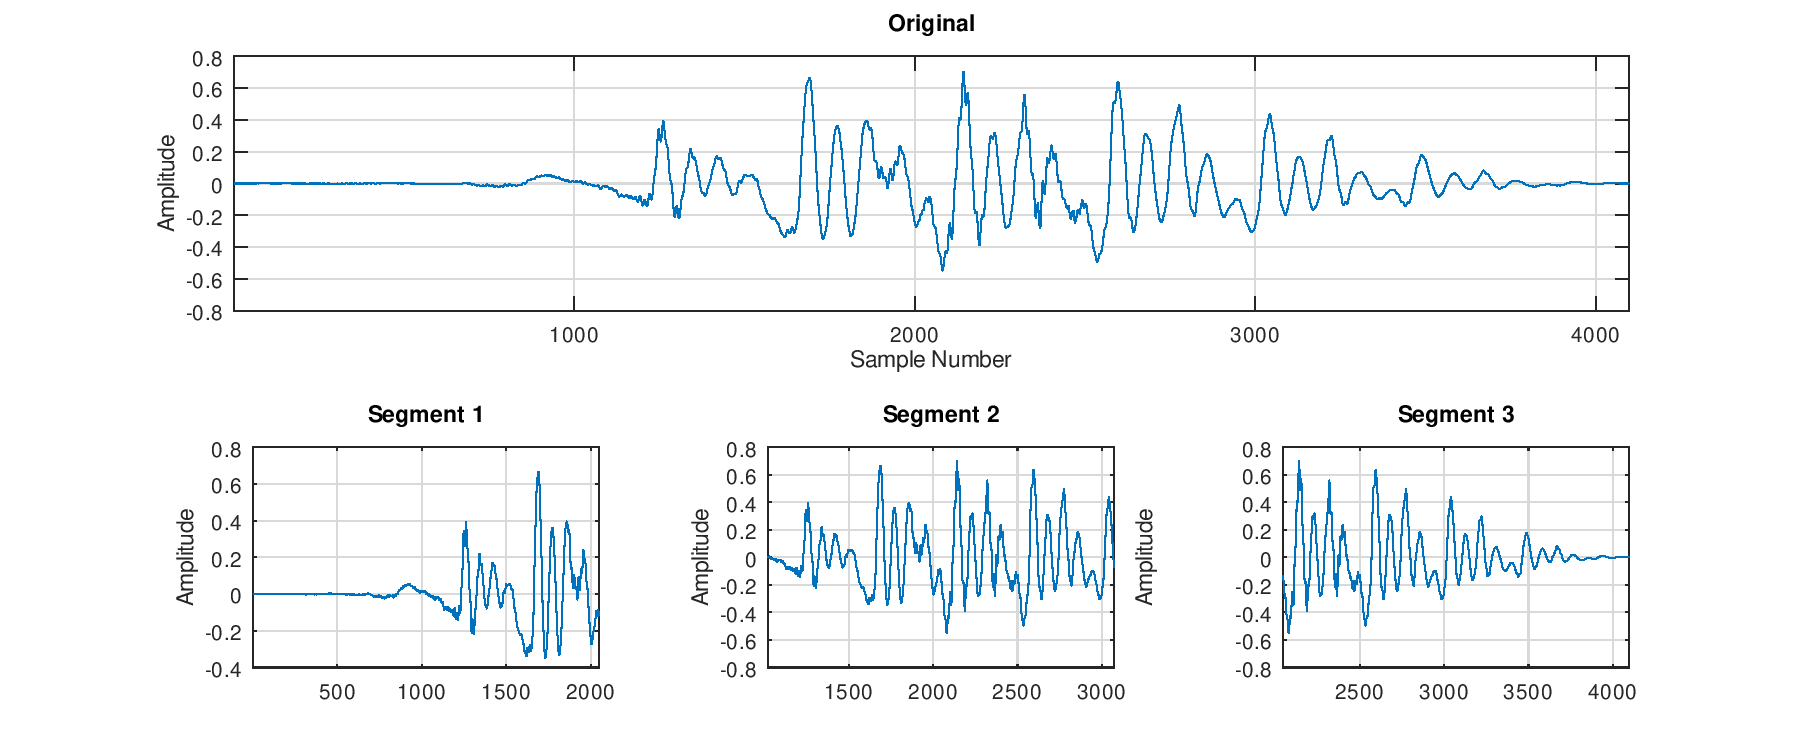
\includegraphics[width=\textwidth, trim={2.5cm 0cm 2.5cm 0cm},clip]
{SegmentationVisualization}
\caption{Segmentation Visualization}
\label{fig:Segmentation}
\end{figure}

There is an obvious trade-off when considering the overlapping percentage. The
more the signal overlaps, the more computational power is needed but it does
usually provide more gradual changes when stitching segments back together. For
this implementation, the overlap percentage was chosen at whatever was most
natural for the pitch shifter(50\% for simple overlap and add and 75\% for the
phase vocoder). A less obvious trade-off is that of segment size. The larger the
segment size, the more latency the system will have but will increase the
fundamental resolution in frequency for the frequency detection and frequency
scaling modules.  Practically the pitch detectors needs al least 2 periods to
calculate the frequency properly, meaning the segment size needs to be at least 1
764 samples long. This corresponds to two periods of a 50Hz signal at 44 100
samples per second. Listing \ref{lst:segment} shows how these segments are
obtained.

\octavelisting{segment}

From this array of segments, it is possible to create the frequency contour. The
basic idea is to pass each segment into the frequency detector, producing a list
of frequencies over time. Unfortunately implementing exactly this would produce
erratic results. The problem comes in when the specified segment is an unvoiced
one. This means no instrument is producing sound in that frame and the frequency
detector will find a frequency based on the background noise. This has been found
to be very high values and can cause issues in the frequency scaler later on. This
is unwanted behaviour and a mechanism is built in to allow the frequency detector
to simply hold the frequency of the previous segment if it regards the segment as
unvoiced. This produces a frequency contour that's much easier to work with.
Listing \ref{lst:getFrequencyContour} shows the Octave implementation of how this
is achieved.

\octavelisting{getFrequencyContour}

It can be seen that a pre-filter is needed for the frequency detector. The filter
is applied in the \colorbox{backcolour}{\lstinline{getFrequencyContour}} function
to allow the frequency detector to only consider individual segments, essentially
allowing for more elegant code. This pre-filter is specific to the frequency
detector and will be discussed more in the frequency detector section.

\section{Target Frequency Contour}

As discussed in the literature review on music theory, the tuning system that will
be used in this pitch correction system is the equal tempered tuning system based
on the interval ratio of $\sqrt[12]{2}$. This tuning system works by choosing a
starting frequency, 440 Hz, and calculating all the other valid frequencies by
successively applying the chosen interval ratio. All the produced frequencies in
the tuning system will be relative to 440 Hz. Listing
\ref{lst:getValidFrequencies} shows how a list of these valid frequencies are
obtained. The list only extends from 55Hz to 3 520Hz but can easily be extended.

\octavelisting{getValidFrequencies}

Now a target frequency needs to be chosen based on the information provided by the
frequency contour and the list of available frequencies. The naive approach would
be to choose the target contour based on the closest pitch contour, as shown in
listing \ref{lst:getClosestFreqContour}. This produces unwanted rapid transitions
when a slightly noisy contour transitions between two notes. Figure
\ref{fig:NoisyContour} shows these unwanted rapid transitions.

\begin{figure}[b]
	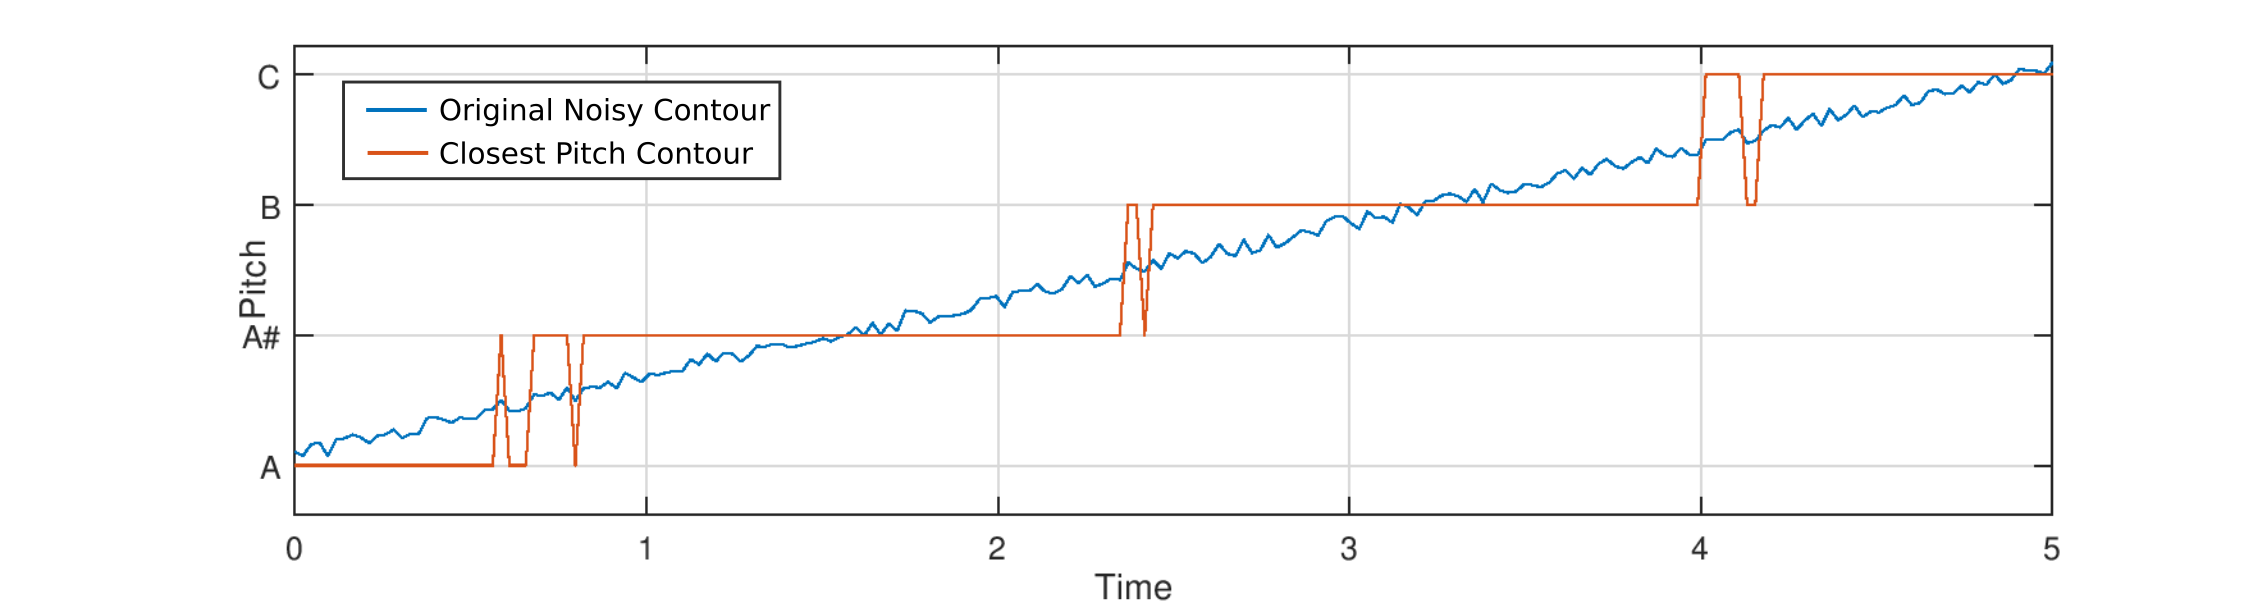
\includegraphics[width=\textwidth,trim={3.5cm 0cm 2.8cm 0cm}]
	{NoisyContour}
	\caption{Rapid Closest Pitch Contour transitions of a noisy Pitch Contour}
	\label{fig:NoisyContour}
\end{figure}

These noisy transitions are common in the field of electrical engineering. The
solution, in the context of electrical engineering, is to use a Schmitt Trigger, a
device that bases it's output, not only on it's current input, but on the previous
output supplied by the device. This dependence on the previous state of the device
is a form of hysteresis and is a common non-linear effect. Listing
\ref{lst:getWantedFreqContour} shows how this Schmitt trigger approach is
implemented in Octave.

\octavelisting{getWantedFreqContour}

The approach is to set a threshold that needs to be exceeded in order to change
the pitch. The exact value of the threshold is a ``tuning value'' and would depend
on the preference of the performer. This ``Schmitt Trigger'' approach produces the
desired affect when the same noisy input contour is applied. This is shown in
figure \ref{fig:NoisyContourFixed}.

\begin{figure}[h]
	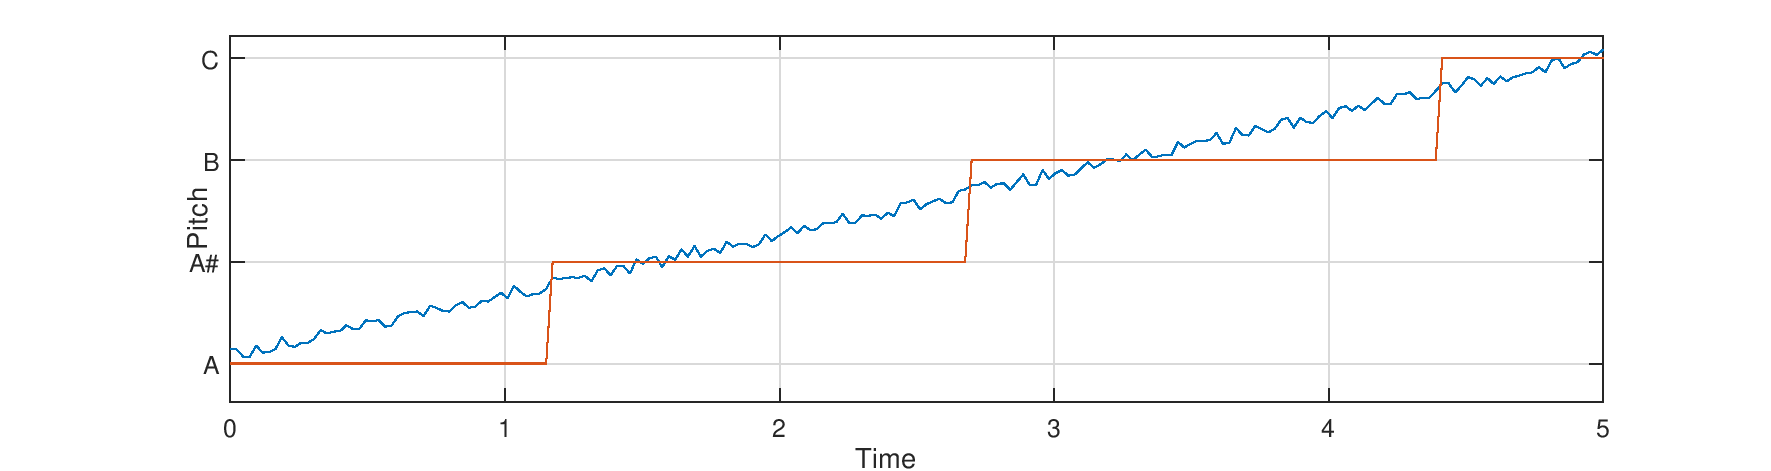
\includegraphics[width=\textwidth,trim={3.5cm 0cm 2.8cm 0cm}]
	{NoisyContourFixed}
	\caption{Result of Schmitt Trigger approach on Noisy Pitch Contour}
	\label{fig:NoisyContourFixed}
\end{figure}

\section{Frequency Detector}

The frequency detector module is the basis for the frequency shifter and it's
accuracy is vital for the success of the whole frequency correction system. Each
implementation has a pre-filter that prepares the signal for the detector.
Thereafter the specific algorithm for frequency detection is applied to each
segment as shown in listing \ref{lst:getFrequencyContour}. The first thing this
algorithm does is determine if the segment is voiced or not. The reason the
presence check is done inside the frequency detector function is because it was
initially thought each detection approach could yield a different approach to a
presence check. This was eventually not investigated further and a single
presence check was used for both algorithms. The presence checking algorithm is
shown in listing \ref{lst:isVoiced}.

\octavelisting{isVoiced}

For now, all the algorithm does is check if the amplitude of the incoming signal
reaches a threshold. This threshold was found empirically and solved the presence
check for all my test recordings. More sophisticated algorithms exist but efforts
were focussed on other modules since this was not deemed the module limiting
performance of the pitch corrector.

\subsection{Zero Crossing Method}

Before the algorithm for the zero crossing method receives the segments, a
pre-processing filter needs to be applied to prepare the frames for the zero
crossing detector. LPC was considered but was found to be quite complicated and a
simpler option suggested by a website\footnotemark\space was implemented. This
involved a low pass filter, to filter out all the harmonic content and noise that
might cause unwanted zero crossings. An 8th order Butterworth filter at 250 Hz was
needed to produce results that contained no errors. The algorithm applied to each
frame is shown in listing \ref{lst:getFrequencyZCM}.

\footnotetext
{\url{https://sound.eti.pg.gda.pl/student/eim/synteza/leszczyna/index_ang.htm}}

\octavelisting{getFrequencyZCM}

The first block in listing \ref{lst:getFrequencyZCM} calls the voicing check
function and only if it return true, continues the algorithm. This is an attempt
to reduce unnecessary computation.  Next, the algorithm uses the built-in Octave
function to find the location of the zero-crossings. The next two blocks relates
to a quirk of the zero crossing method illustrated in figure
\ref{fig:ZeroCrossingRaised}. This figure shows what happens when the segment
under inspection has a slight DC-value.

\begin{figure}[h]
	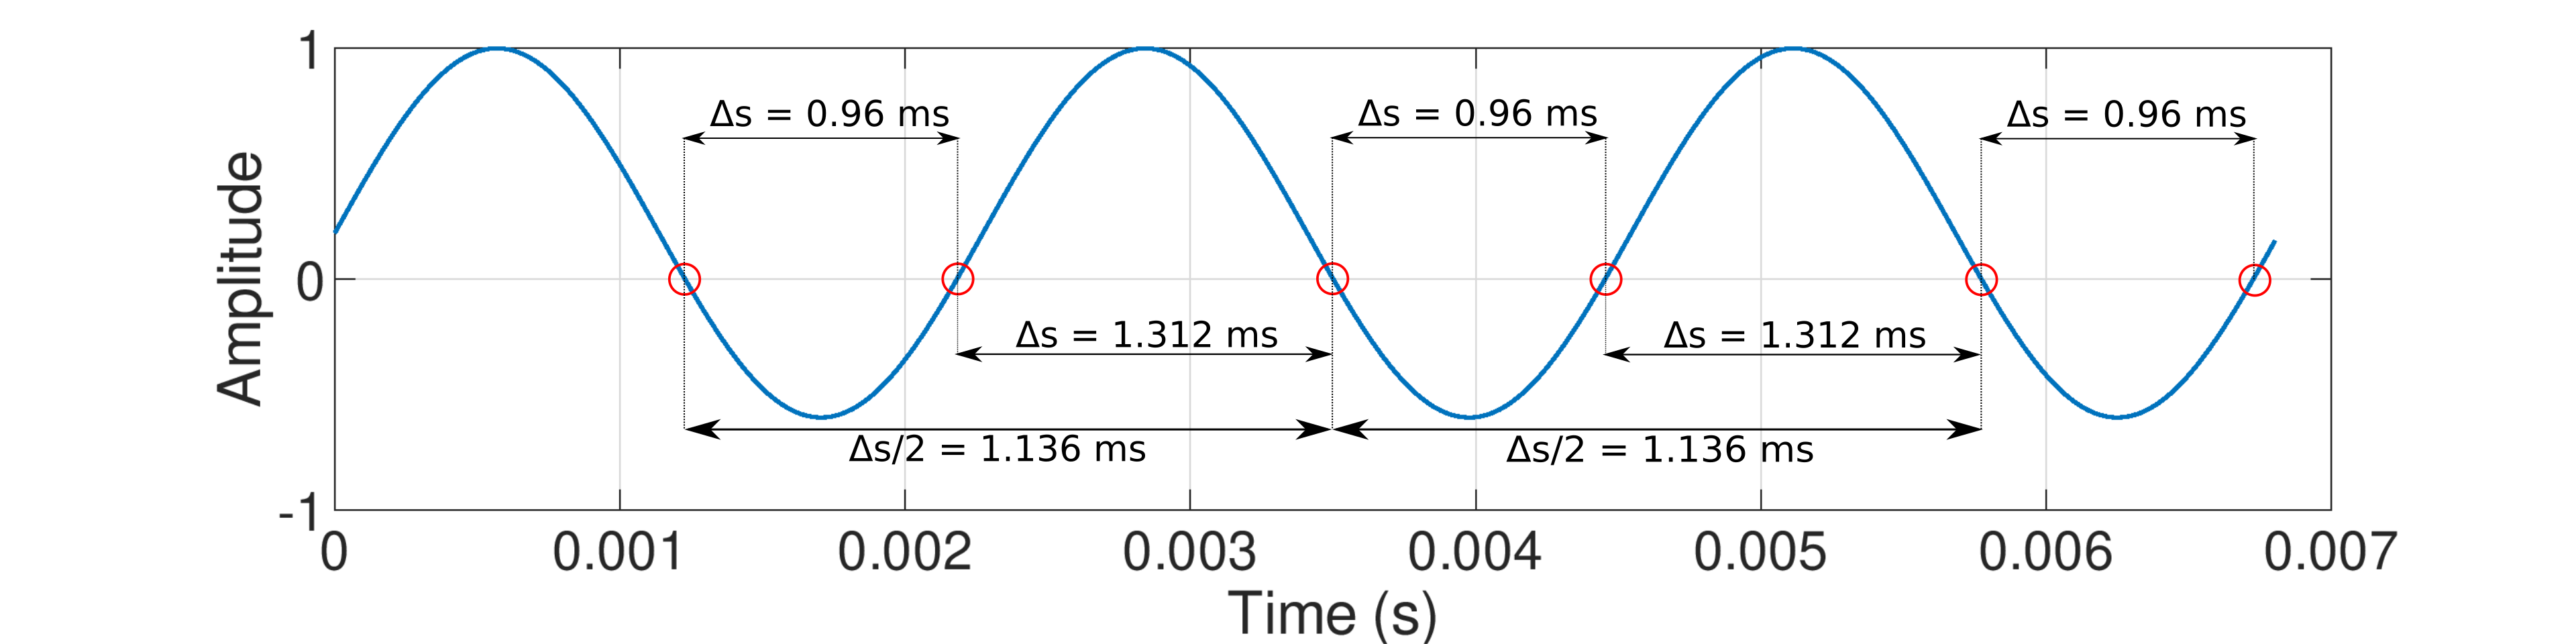
\includegraphics[width=\textwidth,trim={3cm 0mm 3cm 0mm},clip]
	{ZeroCrossingRaised}
	\label{fig:ZeroCrossingRaised}
	\caption{Zero crossing detector on 440 Hz sinusoidal signal}
\end{figure}

The frequency of the signal in the graph is a 440 Hz sinusoid. The formula in
equation \ref{eq:PeriodVsFreq1} requires $\Delta s$ in order to to calculate the
fundamental frequency of the signal. Since the length of $\Delta s$ changes for
each successive zero crossing, using the naive implementation of the formula would
estimate frequencies of 521 Hz and 381 Hz even though the fundamental frequency of
the segment is 440 Hz. Therefore some averaging needs to be done. Averaging two
consecutive $\Delta s$ values would produce the correct result as shown in figure
\ref{fig:ZeroCrossingRaised}. More generally, averaging an even amount of $\Delta
s$ values would produce much more accurate results. This involves ensuring the
considered length of zero crossings is more than three and odd valued. This is
exactly what the Octave implementation does.

\begin{equation}\label{eq:PeriodVsFreq1}
	F_0 = \frac{1}{p} = \frac{1}{2\Delta s}
\end{equation}

The second to last block of code gets the length of the region from the first to
the last zero crossings considered. This is going to be the region being averaged.
The last block calculates the frequency from the information of the amount of
zero crossings considered and the length of the region considered. With this
algorithm, an estimate of the fundamental frequency for a segment can be
calculated.

\subsection{Autocorrelation Method}

As with the zero crossing method, a pre-possessing LPF is applied. It was found
that this filter did not need as strict parameters and was set to 900 Hz. This was
on the recommendation in the paper comparing pitch detection
methods\cite{ComparitivePitch}. This was found to be sufficient for all testing
recordings.

Before the auto-correlation method could be implemented, a center clipping
function needed to be written. This center-clipping is needed to remove harmonic
content and formants but retain the fundamental periodicity of the signal. Listing
\ref{lst:clip} shows the implementation of this clipping function. This is a
straight forward implementation and the code is considered self explanatory.

\octavelisting{clip}

Now that a center-clipping function has been written, the autocorrelation approach
to frequency detection is implemented. The Octave code is shown in listing
\ref{lst:getFrequencyAutoCorr}. A voice checking, as in the zero-crossing method,
is done first. Thereafter the signal needs to be center-clipped. The literature
review suggested taking the maximum value of the first and third part of the
segment and scaling that by 0.67. The reason for only considering the first and
last third is not fully understood and the decision was made to consider the whole
segment. Now the clipped signal is autocorrelated. The peaks of this
auto-correlated signal needs to be found using a built-in Octave function. The
\colorbox{backcolour}{\lstinline{findpeaks()}} function requires the input to be
greater than 0. All the peaks int the second half, greater than 80\% of the center
peak, are returned.  The distance to the second peak is considered the period of
the signal.

\octavelisting{getFrequencyAutoCorr}

To demonstrate the function of the center clipping, figure \ref{fig:ClipVsNoDemo}
shows the result of the same segment with and without the clipping applied. The
segment is of a vocal recording containing all the formants and harmonics a signal
is expected to contain.

\begin{figure}[h]
	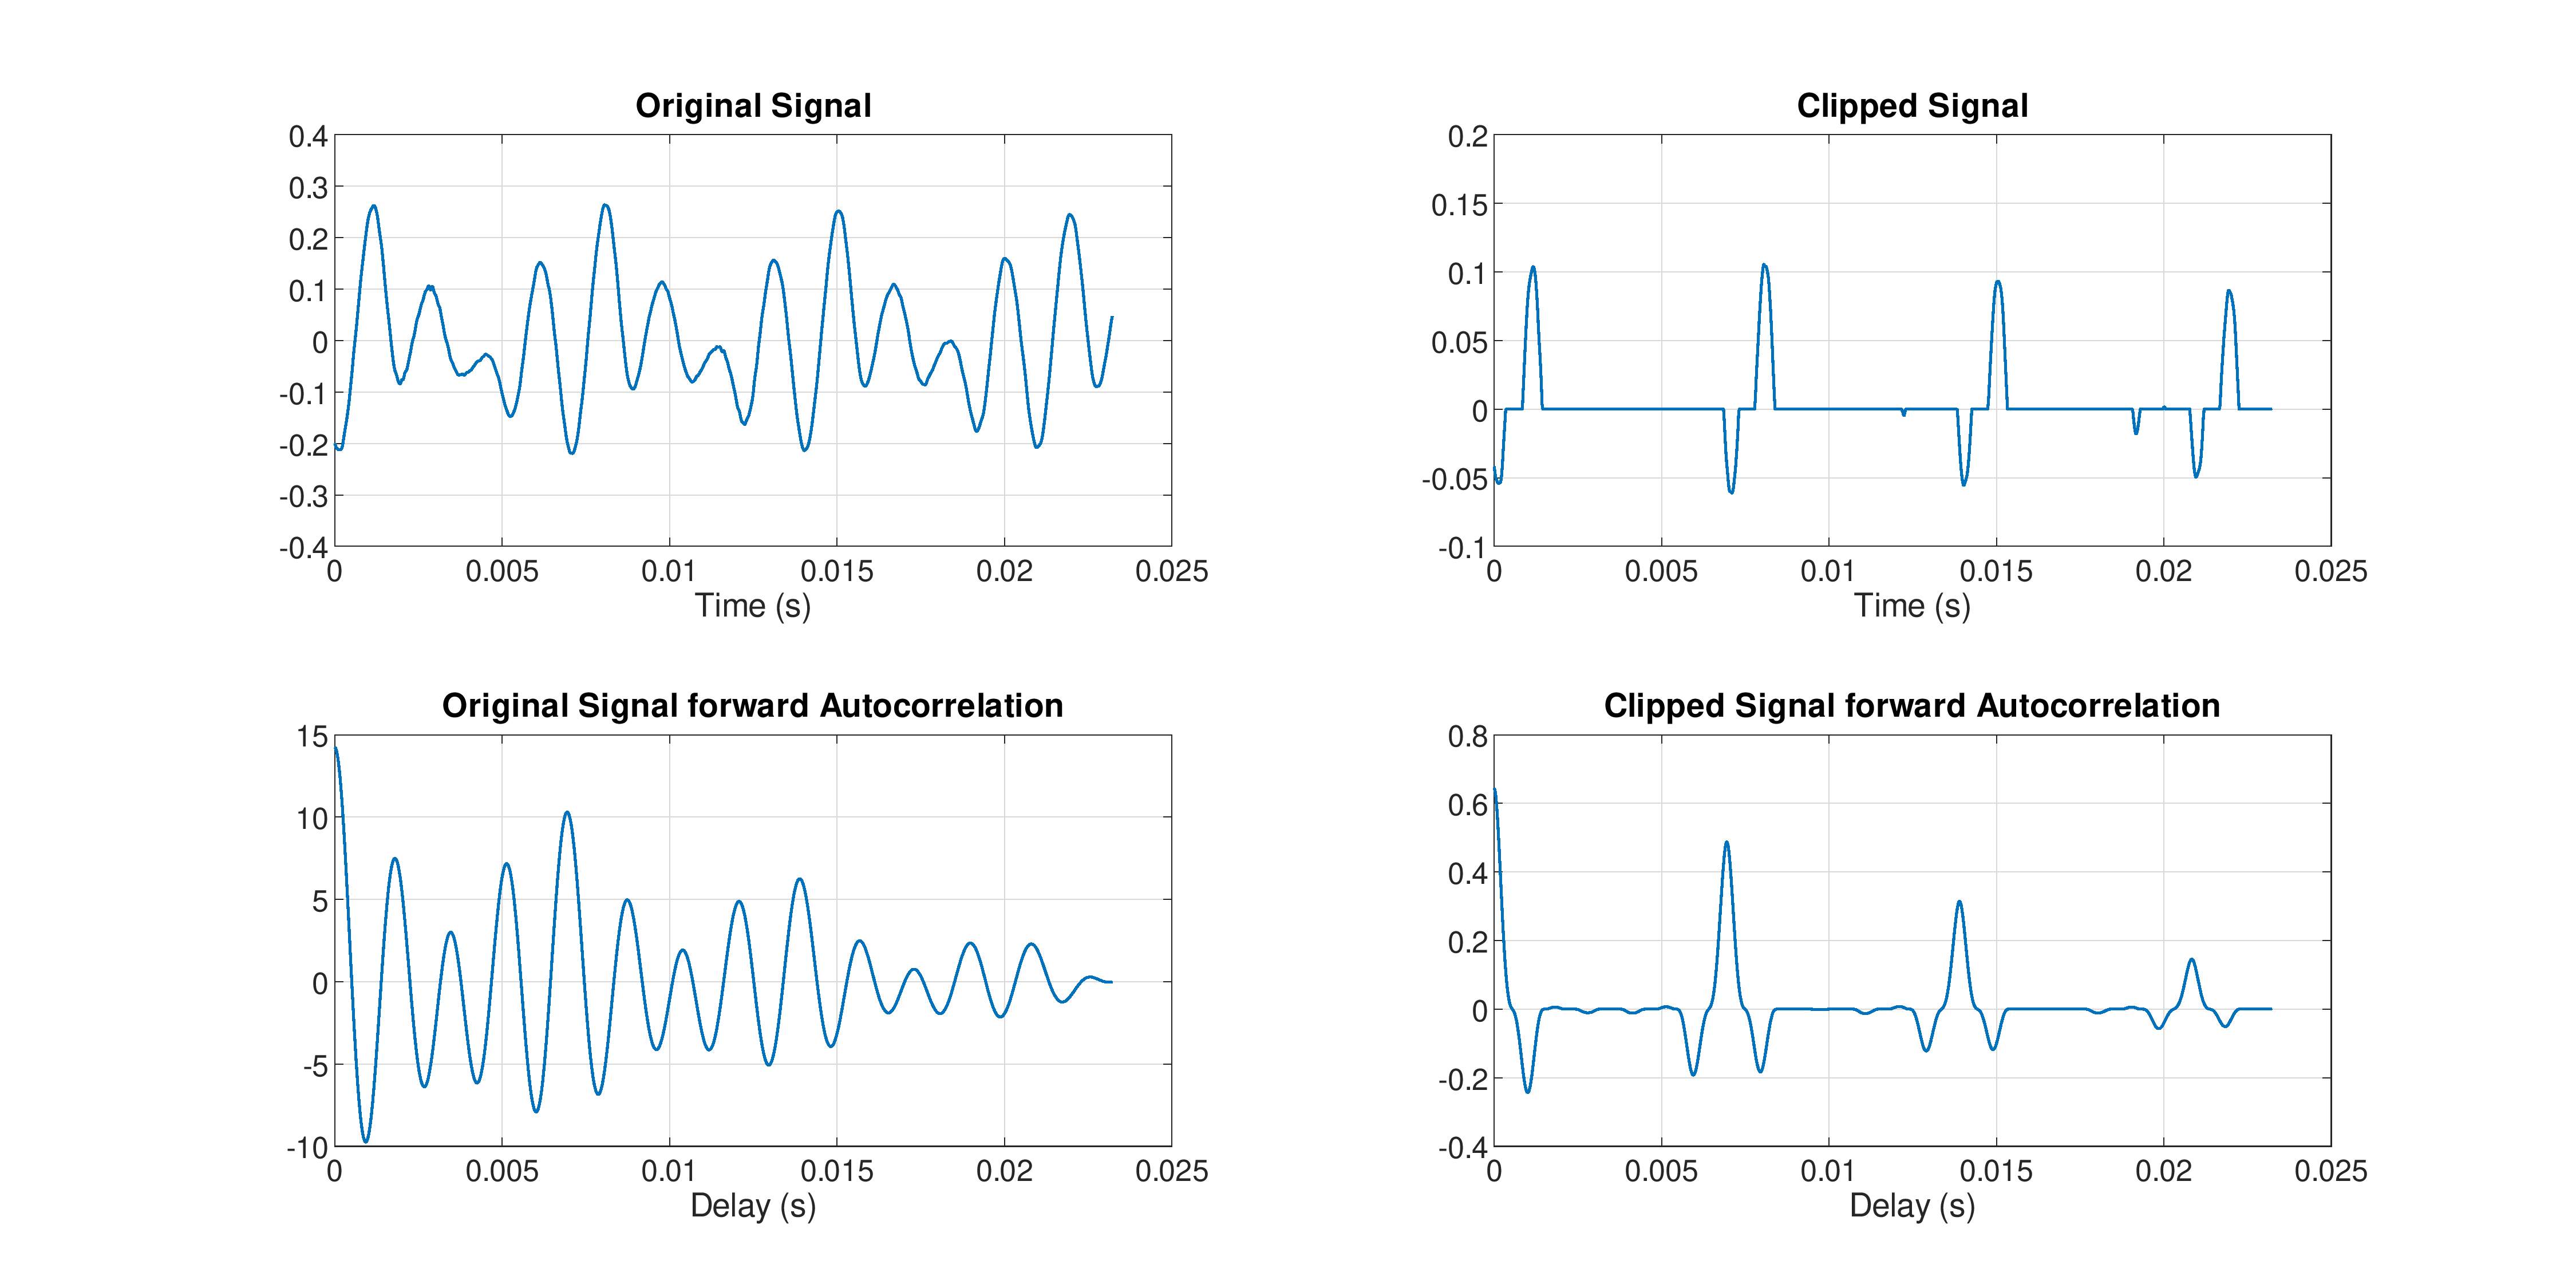
\includegraphics[width=\textwidth,trim={3cm 0mm 2.5cm 0mm},clip]
	{ClipVsNoDemo}
	\label{fig:ClipVsNoDemo}
	\caption{Zero crossing detector on 440 Hz sinusoidal signal}
\end{figure}

Below is the result of the second half of the autocorrelation function of the
clipped and non-clipped signal. The distance from the value at zero delay and the
first peak is the period of the signal. The figure makes is obvious that center
clipping produces a less ambiguous period. Further testing could to be done to
calculate the ideal values for the clipping threshold and peak finding threshold.
The chosen values of 0.6 and 0.8 respectively, was considered to perform good
enough and time was spent working on other parts of the pitch correction system.

\section{Frequency Scaler}

The frequency scaler was considered the most difficult module in the pitch
correction system. In-depth understanding needed to be acquired before anything
worked at all. A test was devised to see if the pitch shifter improved. The test
was to scale a 220 Hz sinusoid sound wave, five seconds in duration, up and down
by 50\% according sin function of a two and a half second period. The quality of
this scaled 440 Hz pitch was listened to and changes were made depending on
intuition gained from the listening experience. This evaluation method can not be
considered a rigorous metric but was found to be very useful in the development of
the algorithms.

\subsection{Simple Overlap and Add}

The simple overlap and add method was understood first but actually implemented
after the phase vocoder. This was because it was not regarded as a serious
approach. This intuition was correct, as will be shown. The merit for including
this method is to illustrate it's shortcomings and to be a precursor for the
synchronized overlap and add method used by most pitch shifters. Unfortunately the
synchronized overlap and add approach was not implemented due to time constraints.
This method feels a bit like a useless appendage but should still be considered a
stepping stone and reference point to proper methods.

The Octave code of this method is cumbersome and a straight forward implementation
of what is described in the literature review. For this reason the implementation
code for this method is added in Appendix C. Instead of discussing the Octave
code, the results of the frequency scaler will be inspected.

\begin{figure}[h]
	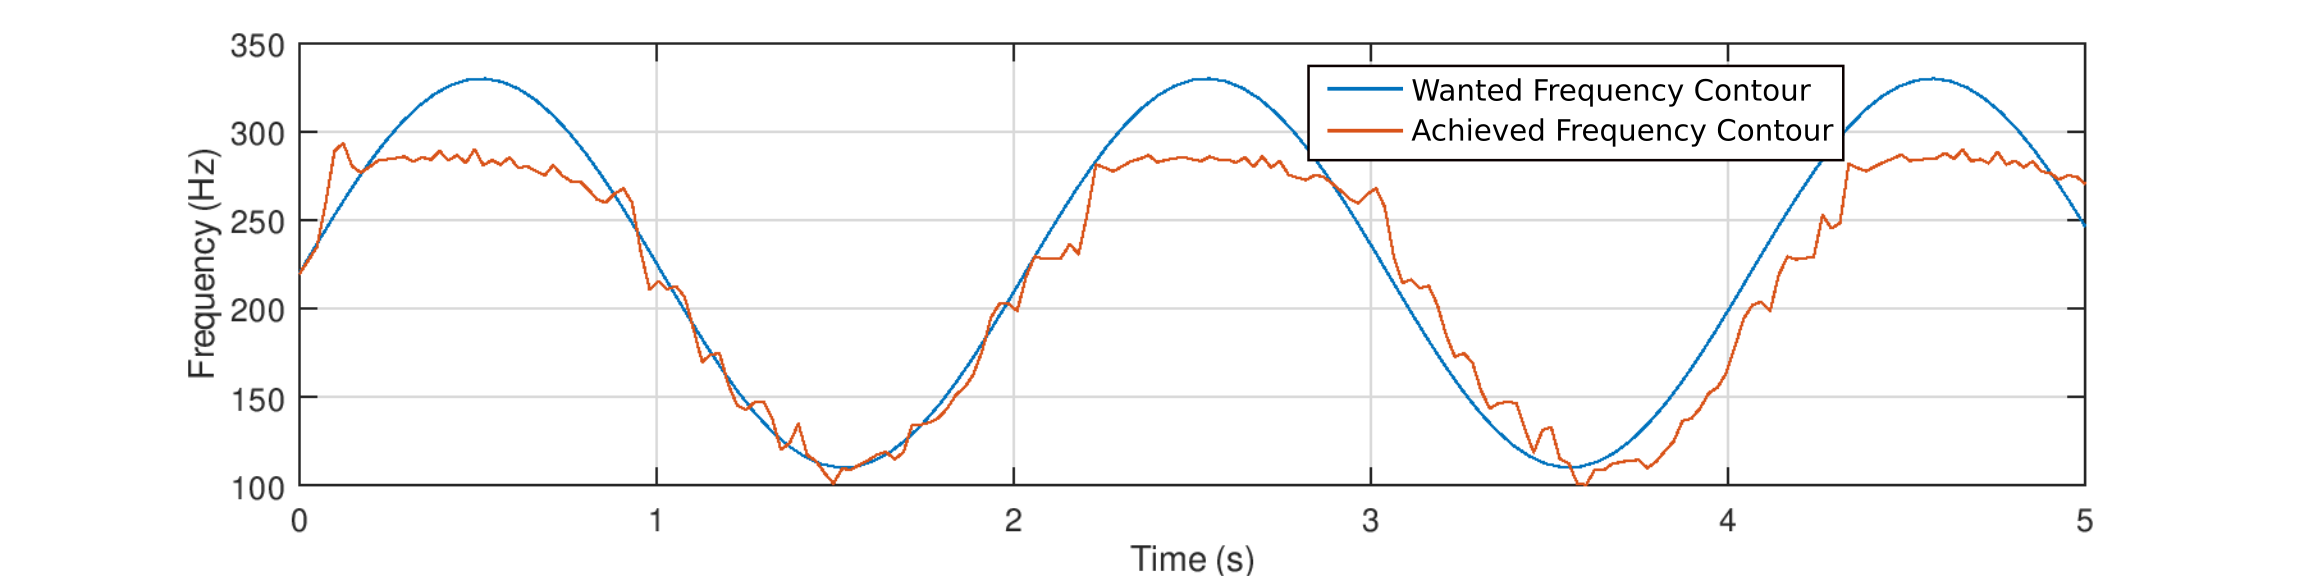
\includegraphics[width=\textwidth,trim={2.5cm 0mm 2.5cm 0mm},clip]
	{TestScalingOLA}
	\caption{Scaling Test of Simple Overlap and Add Algorithm}
	\label{fig:ScalingTestSOLA}
\end{figure}

From figure \ref{fig:ScalingTestSOLA} it can be seen that somewhat pitch shifting
is achieved. This is not nearly good enough for a high-fidelity application, but
is a step in the right direction. Some aspects to point out on figure
\ref{fig:ScalingTestSOLA} is that the algorithm seems to have trouble with scaling
to a higher frequency. The achieved contour follows the wanted contour much closer
on the downward section. What's happening here is slightly misleading, or rather,
not the full story. The frequency scaler seems to achieve scaling in discrete
steps. These are log frequency steps, or alternatively, pitch steps. Figure
\ref{fig:ScalingTestSOLAPitch} shows the same plot, except with pitch on the
y-axis. Here it can be seen that the pitch shifting algorithm has a resolution of
3 semitones. The goal of the pitch shifter is to shift pitch within a
semitone, making this pitch shifter not nearly good enough.

\begin{figure}[h]
	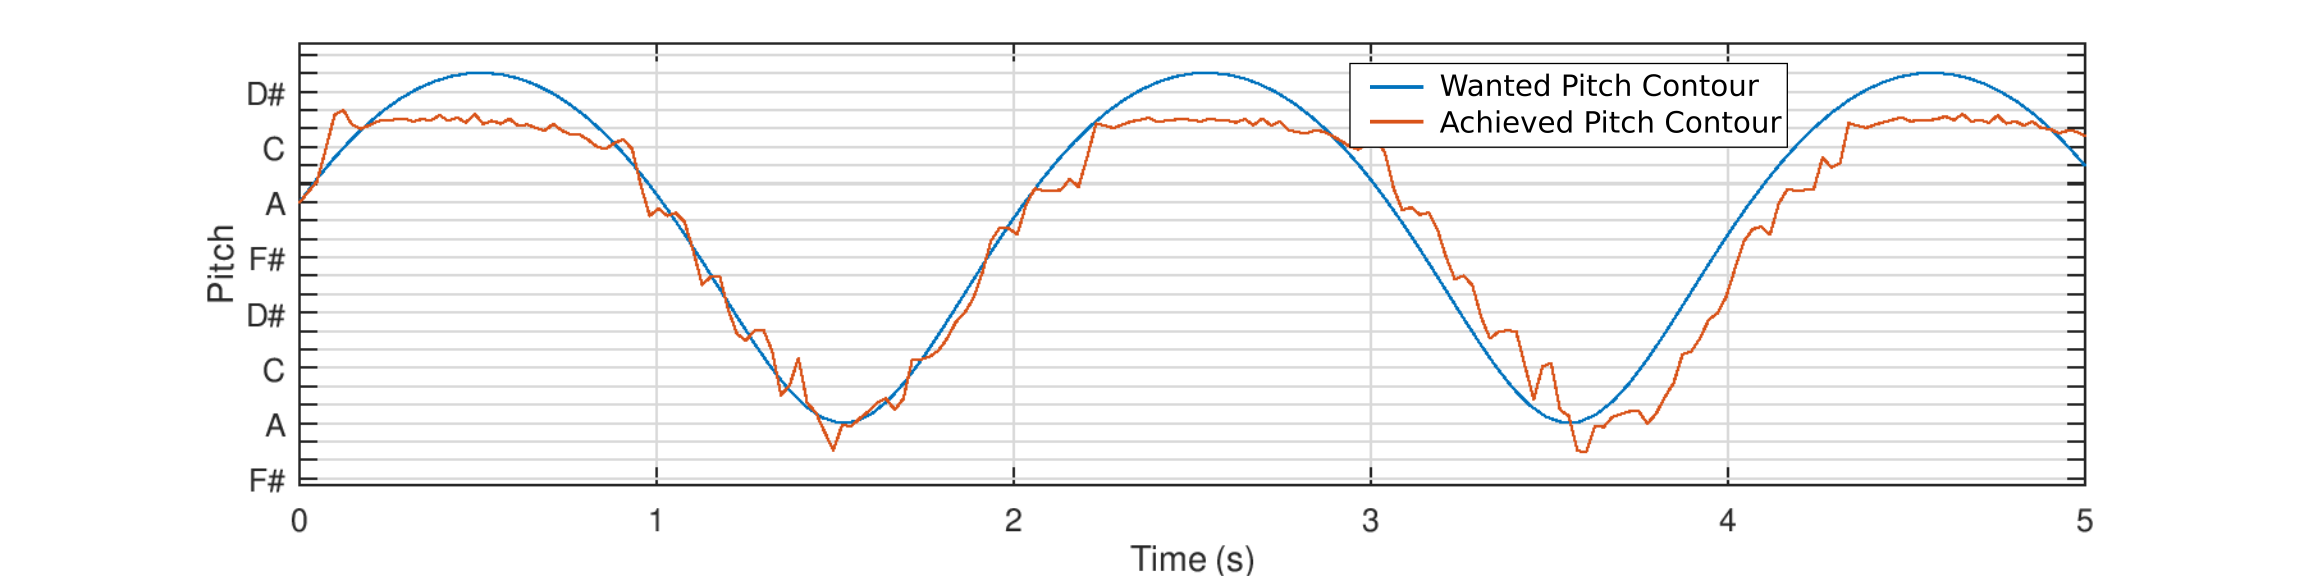
\includegraphics[width=\textwidth,trim={2.5cm 0mm 2.5cm 0mm},clip]
	{TestScalingOLAPitch}
	\caption{Pitch graph of figure \ref{fig:ScalingTestSOLA}}
	\label{fig:ScalingTestSOLAPitch}
\end{figure}

\subsection{Phase Vocoder}

The Phase vocoder was the most interesting algorithm investigated. The details of
how the approach works has been explained in the literature review. The
implantation Dan Ellis provides on his
website\footnote{\url{http://www.ee.columbia.edu/ln/rosa/matlab/pvoc/}} was used.
Other implementations were also inspected, but the one provided by Professor Ellis
was the cleanest, simplest approach. The implementation itself will not be
explained but rather the interface provided will be explained. It will be viewed
as a library, equivalent to the other Octave functions provided built in. The
Octave code needed to implement arbitrary pitch shifting, using this library, will
be explained.

\vspace{1cm}
The phase vocoder implementation consists of three functions:
\vspace{-1cm}
\begin{itemize}
\item\colorbox{backcolour}{\lstinline{stft(x, f, w, h, sr)}}\newline
A function that receives a signal x, does f-point FFT's on w-sized windows spaced
h samples apart and returns a form of STFT that the rest of the library knows how
to deal with.
\item\colorbox{backcolour}{\lstinline{pvsample(b, t, hop)}}\newline
A function that receives a STFT array b, a new time-base t, and a hop size h,
and returns a STFT array, re-sampled at the new time-base according to the phase
vocoder algorithm.
\item\colorbox{backcolour}{\lstinline{istft(d, ftsize, w, h)}}\newline
A function that receives a STFT array d, with a FFT size specified by ftsize,
window size specified by w, hops size specified by h and returns a signal created
by an overlap and add method from the IFFT's of the STFT frames.
\end{itemize}

The website suggests values for the window size and fft size of 2 048 and 512
respectively and that the functions be executed in the order shown above. The only
input to really consider is the new timebase t. The normal timebase is the
integer values, starting from zero and having a length equal to the amount of STFT
frames. Providing an array t, of 0.5 unit increments and executing the code is
equivalent to stretching the input recoding by a factor of two. Re-sampling this
recording at half the original sampling rate will cause all the frequencies to be
scaled by a factor of two and now the sample will have a length equal to the
original. This is how pitch shifting by a constant factor is achieved using the
phase vocoder.

The timebase, however, does not need to be spaced equally. It can be spaced at
arbitrary intervals. The re-sampling operation can also be done arbitrarily using
spline interpolation. This theoretically allows one to scale the frequency by an
arbitrary time dependent factor. This is exactly what we require for pitch
correction. The function indication the time dependent scaling factor is referred
to as the scaling ratio contour. This algorithm is shown in listing
\ref{lst:getScaledSamplePV}

\octavelisting{getScaledSamplePV}

\begin{figure}[h]
	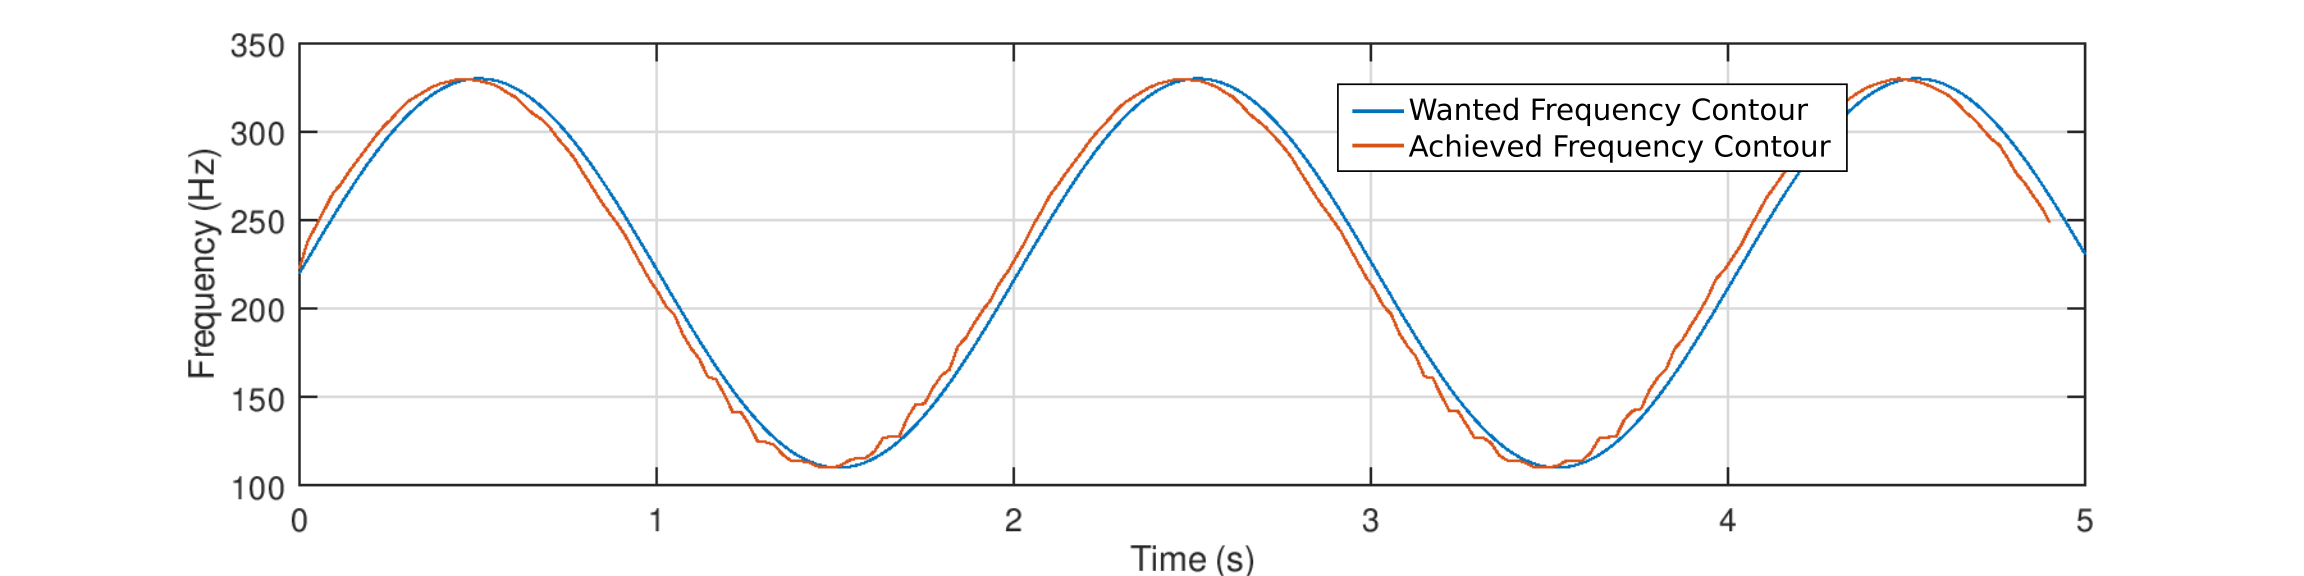
\includegraphics[width=\textwidth,trim={2.5cm 0mm 2.5cm 0mm},clip]
	{TestScalingPV}
	\caption{Scaling Test of Phase Vocoder}
	\label{fig:ScalingTestPV}
\end{figure}

\begin{figure}[h]
	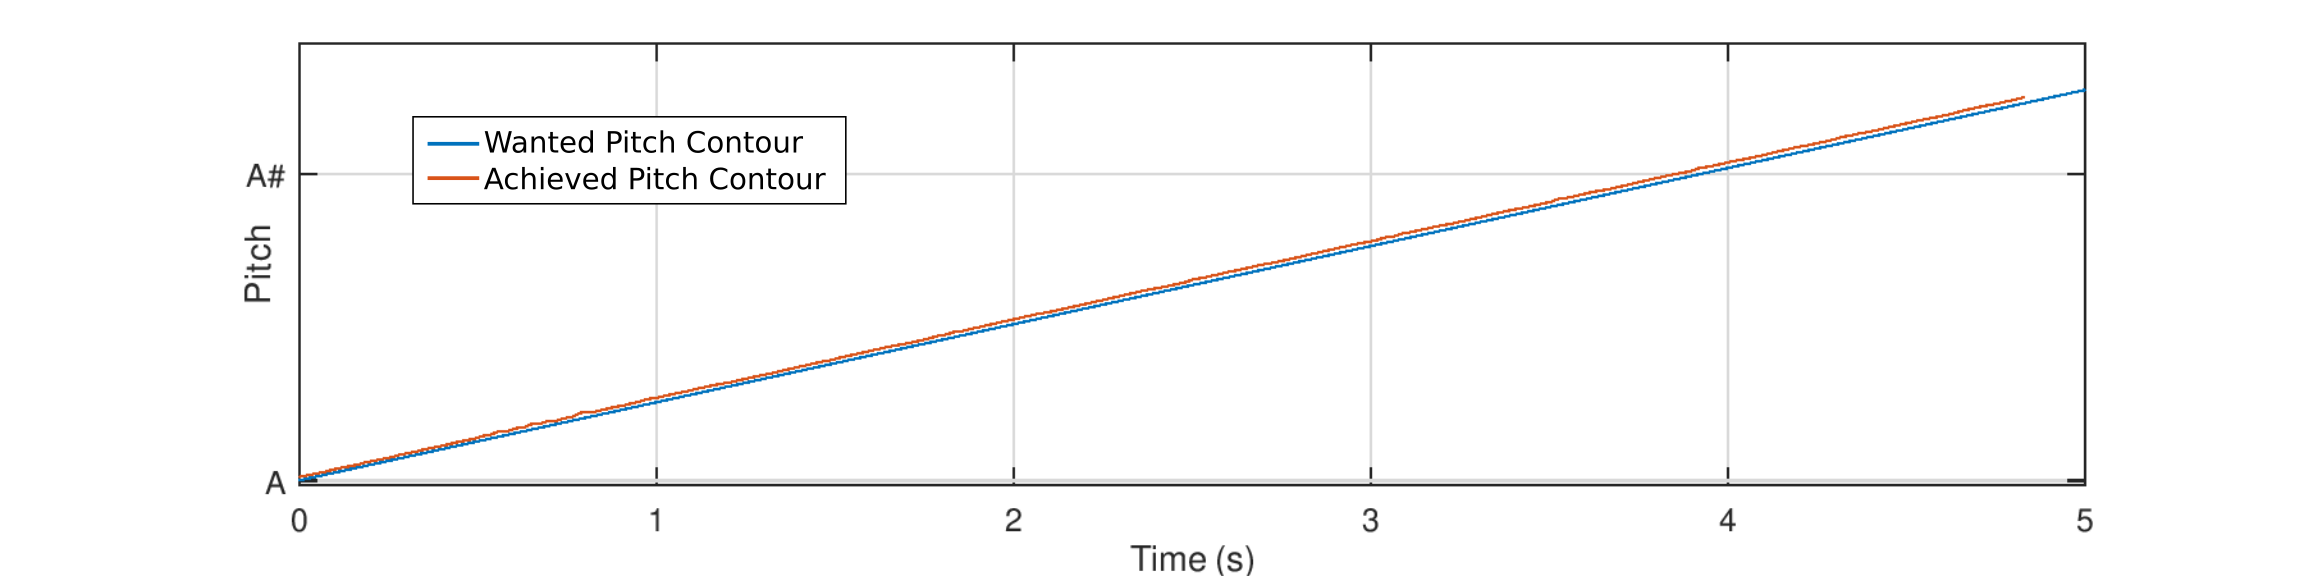
\includegraphics[width=\textwidth,trim={2.5cm 0mm 2.5cm 0mm},clip]
	{TestScalingPVPitch}
	\caption{Pitch Resolution of Phase Vocoder}
	\label{fig:ScalingTestSOLAPVPitch}
\end{figure}

\color{red}
To do:
\begin{itemize}
	\item Describe method in more detail than lit review
	\item Show snips of code and graphically what it's doing
	\item Show performance metrics
\end{itemize}
\color{black}

\section{Pitch Corrector}

\color{red}
To do:
\begin{itemize}
	\item Describe which modules were added put together
	\item Describe why each module was chosen
	\item Describe each system and show its performance
\end{itemize}
\color{black}

\section{Concept Expansion}

\color{red}
To do:
\begin{itemize}
	\item Explain that more cool stuff were found
	\item Post Correction
	\item Harmonization
	\item Pitch Scaling by a Constant Factor
\end{itemize}
\color{black}
